\chapter{Theory}
\label{sec:theory}

\section{Design Load Cases}
The user must specify the metocean conditions that drive the wind and
wave loads upon the floating substructure.  Ideally, multiple metocean
conditions would be used for design optimization, many of which have
already been codified \citep{iec2009}.  This includes standard operating
conditions that determine fatigue loads, maximum allowable operating
conditions (e.g. max thrust), maximum survivable conditions, and likely
others that bound a design.  As of this writing, \textit{FloatingSE}
only supports execution and optimization around a single metocean
condition and load case.  Future development will enable optimization
against a vector of load cases, likely those used in code standards.

\section{Load Path}
Similar to the assumptions in \textit{JacketSE}, as stated by
\citep{JacketSE}, the primary simplification in \textit{FloatingSE} is
the treatment of all loads as pseudo-static. This approximation reduces
computational time and resources, since an accurate calculation of
dynamic loads requires more sophisticated numerical tools and
simulations.  Thus, users must exercise care in selecting loads and
safety factors to compensate for the lack of a fully dynamic treatment.
Furthermore, fatigue effects and structural lifetime estimates are also
not currently calculated, but could be incorporated in future
developments.  In general though, fatigue loading tends to dominate the
design of joints, flanges, and welds in a design (which are not
prominently featured in \textit{FloatingSE}), whereas overall structural
sizing of the main shell geometry is driven by modal and
buckling-strength requirements (which are prominently featured in
\textit{FloatingSE}).

A floating wind turbine undergoes loading from a number of sources.  The
primary loading source for the tower comes from the aerodynamic loads
induced by the rotor. The substructure must resist the combination of
both rotor loads and hydrodynamics loads, with the latter becoming more
and more important as water depth and wave heights increase.
\textit{FloatingSE}, together with other WISDEM modules, accounts for
these two dominant load sources, as well as the self-loading of gravity
loads.  Other sources of loading, such as installation loads, accidental
loads, vortex-induced vibrations, ice, and seismic loads are ignored.

Aerodynamic and hydrodynamic loads are computed within
\textit{FloatingSE} and \textit{CommonSE}.  Rotor thrust loads are
computed in \textit{RotorSE}, and imputed into \textit{FloatingSE} as
inputs.  Loading over the entire turbine is then assembled within
\textit{FloatinSE} for a structural analysis by Frame3DD (via
\textit{pyFrame3DD}).  Once all member loads and stresses are
determined, compliance checks against international standards are
evaluated and can be used as design constraints during optimization
runs.

\subsection{Wind and Wave Loads}
Wind drag loads are applied to the tower body and the upper part of the
substructure that extends above the waterline.  They are not applied to
connecting truss members that may be part of the substructure geometry.
These drag loads are computed assuming the tower and columns are smooth
circular cross-sections and that the drag coefficient can be selected as
a function of the flow Reynolds number \citep{Roshko}.  The calculations
of the wind and wave loads are provided by multiple modules within
\textit{CommonSE}.

For the tower and portion of the substructure that extends above the
waterline, wind loading arises from the aerodynamic drag on the
structure.  This drag changes with height, since the wind profile and
cross-sectional geometry varies.  WISDEM allows the user to select from
a power-law or logarithmic scaling of wind with height, where the
power-law approximation is given by,
\[
  U_a(z) = U_{ref}\left(\frac{z}{z_{ref}}\right)^{\alpha}\quad,
\]
where $U_a(z)$ is the wind velocity as a function of height, $U_{ref}$ is a
reference wind speed measured at a reference height, $z_{ref}$, and
$\alpha$ is the shear exponent used in the power-law approximation of
wind profiles.  The wind profile then feeds the aerodynamic drag,
Reynolds number, and drag coefficient,
\begin{equation} \label{eqn:drag}
  dF(z) = \frac{1}{2} \rho_a U_a^2(z) d(z) c_d(Re) dz;\qquad
  Re_d = \frac{\rho_a U_a(z) d(z)}{\mu_a}\quad,
\end{equation}
where $Re_d$ is the Reynolds number based on diameter, $\rho_a$ and
$\mu_a$ are the density and viscosity of air, $d(z)$ is the diameter of
the column as a function of height, $c_d$ is the 2-D drag coefficient, and
$dF(z)$ is the force per unit length in the z-direction.

Wave drag loads arise from similar processes, but are computed using
Morison's equation to account for the different fluid properties and
dominant physics relative to air.  Morison's equation is a
semi-empirical expression, as opposed to a model of a specific physical
process, that predicts the total hydrodynamic loads.  It is comprised of
two components, one for viscous drag contributions and another for
inertial effects (which includes incident, diffracted, and radiated wave
effects).  For flow past structures with circular cross sections,
Morison's equation for force per unit length ($dF(z)$) takes the form,
\begin{equation} \label{eqn:morison}
  dF(z) = \frac{\pi d^2(z)}{4} \rho_w C_m \dot{U}_w(z)dz + \frac{1}{2} \rho_w U_w^2(z) d(z) c_d(Re)dz\quad,
\end{equation}
where $C_m$ is the added mass coefficient (assumed to be $C_m=2$),
$U_w(z)$ is the current speed as a function of height, $\dot{U}_w(z)$ is
the acceleration as a function of height, and the Reynolds number is
computed by substituting in the appropriate properties for water,
\[
Re_d = \frac{\rho_w U_w(z) d(z)}{\mu_w}\quad.
\]

To compute Morison's equation, expressions for local fluid velocity and
acceleration are required.  Wave particle velocity (not the same as the bulk
velocity of the wave) is assumed to follow linear (Airy) wave theory
\begin{equation} \label{eqn:Uwave}
U_w(z) = a\omega\frac{\cosh\left[\kappa\left(z + D \right)\right]}{\sinh\left(\kappa D\right)}\cosh\left(\kappa x -
  \omega t\right);
\qquad \omega=\frac{2\pi}{T} = \sqrt{ g \kappa \tanh\left(\kappa
    D\right) } \quad,
\end{equation}
where $\omega$ is the circular frequency, $T$ is the wave period, $a$ is
the wave amplitude (half of the significant wave height), $D$ is the
total water depth, $g$ is the acceleration of gravity, and $\kappa$ is
the wave number numerically computed from the dispersion relationship
given as the last expression in Equation \ref{eqn:Uwave}.  Note that the
horizontal particle velocity varies in time and space (by the
$\kappa x - \omega t$) term.  Thus, the individual particles in the wave
are also accelerating at different rates,
\begin{equation} \label{eqn:Awave}
\dot{U}_w(z) = a\omega^2\frac{\cosh\left[\kappa\left(z + D \right)\right]}{\sinh\left(\kappa D\right)}\sinh\left(\kappa x -
  \omega t\right)\quad.
\end{equation}
For
simplicity, \textit{FloatingSE} only considers the maximum velocity and
acceleration at a given height, and makes a conservative assumption that
they occur concurrently in time and space.  This essentially means ignoring the
$\kappa x - \omega t$ term, since the maximum of any hyperbolic sine or cosine
term is one.



\subsection{Rotor Nacelle Assembly (RNA) Loads}
From a quasi-steady-state point of view, the RNA loads reduce to three
forces and three moments along the main coordinate axes
\citet{JacketSE}. The thrust is the biggest force responsible for the
bending moment distribution along the tower and loads on the
substructure.  There is the additional effect of the gravitational load
caused by the offset of the RNA center of mass from the tower
centerline.  This effect is more pronounced for downwind turbines than
upwind turbines, but is included regardless.

\textit{FloatingSE} does not compute the force and moment components
directly, but rather accepts them as inputs from other WISDEM modules or
from the user directly.  The methodology and fidelity in the RNA loads
calculation are addressed in \textit{RotorSE} and \textit{DriveSE}.


\subsection{Loads Integration and Structural Analysis}
The analysis tool, Frame3DD, is an open-source tool for static and
dynamic structural analysis of 2-D and 3-D frames and trusses with
elastic and geometric stiffness. It computes the static deflections,
reactions, internal element forces, natural frequencies, and modal
shapes using direct stiffness and mass assembly \citep{frame3dd}.  The
WISDEM toolkit developed a python interface, \textit{pyFrame3DD}, to
avoid the use of intermediate input and output text files.  All of the
loads integration happens within Frame3DD, where the whole floating
turbine load path, from the rotor to the keel of the substructure, is
modeled with simple Timoshenko frame elements \citep{timoshenko}.

\subsubsection{Discretization}
Long slender components, such as the tower and substructure columns, are
broken up into a finer discretization than the physical ``cans'' that
they are actually made of.  This finer discretization gives greater
resolution of internal forces and natural frequencies.  Substructure
pontoons are represented as single frame elements.  Frame elements are
described by their cross sectional properties (area, moments of inertia,
modulus of elasticity, and mass density) and starting and ending nodes.
For simple geometries, such as pontoons with tubular cross sections,
these properties are straightforward calculations.  For the turbine
tower, tubular cross section properties are also used, albeit at a finer
discretization.  For substructure columns, which may have permanent or
variable ballast and bulkheads, it is assumed that these extra features
are not load-bearing, so tubular cross section properties are also used.
However, the material mass density of the frame element is scaled to
reflect the true mass of the whole section, including ballast, to ensure
that gravity loads are captured correctly.  Thus, for the tower,
columns, and pontoons, only cylindrical (tubular) cross-sections are
supported for now.  Future development may support other cross-sectional
geometries.  For the tubular cross sections, the critical properties
needed by Frame3DD given user inputs of diameter, $d$, and tube (or
wall) thickness, $t$, are,
\begin{align*}
  \textrm{Outer radius, } r_o &= d/2\\
  \textrm{Inner radius, } r_i &= r_o - t\\
  \textrm{Material area, } A &= \pi \left( r_o^2 - r_i^2 \right)\\
  \textrm{Bending second moment of area, } I_{xx} &= I_{yy} = \frac{\pi}{4}\left( r_o^4 - r_i^4 \right)\\
  \textrm{Torsion second moment of area, } I_{zz} &= J_0 = I_{xx} + I_{yy}\\
  \textrm{Shear area, } A_{s} &= A / \left[ 1.124235 + 0.055610\left(\frac{r_i}{r_o}\right) +
           1.097134\left(\frac{r_i}{r_o}\right)^2 - 0.630057\left(\frac{r_i}{r_o}\right)^3 \right]\\
  \textrm{Bending modulus, } S &= I_{xx} / r_o \\
  \textrm{Torsion modulus (shear constant), } C &= I_{zz} / r_o
\end{align*}
Note that the shear area expression is an empirical relationship as
opposed to an analytical expression.

\begin{figure}[htb]
  \begin{center}
    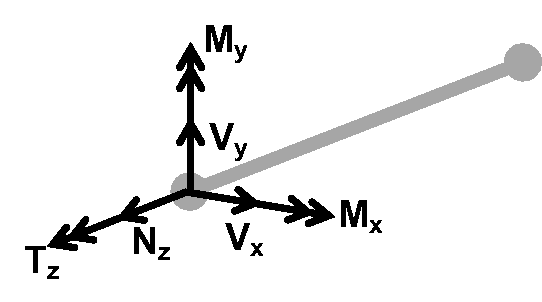
\includegraphics[width=2in]{figs/frameCS.pdf}
    \caption{Coordinate system for frame element forces.}
    \label{fig:frameCS}
  \end{center}
\end{figure}

\subsubsection{Loads}
The forces, moments, and mass properties of the rotor-nacelle assembly
(RNA) are inputs to \textit{FloatingSE} (mass properties are assumed to
be relative to the tower top position).  It assumed that the RNA is a
rigid body with respect to the tower modes and the mass properties,
forces, and moments, are applied to the corresponding node in the model.
The forces along each mooring line are applied upon their connection
point nodes on the structure.  The wind and wave forces per unit length
in Equations \ref{eqn:drag} and \ref{eqn:morison} are applied as
trapezoidally varying loads along the column elements.  Other loads
applied to the structure include the gravity loads, and the buoyancy
acting on the submerged elements.

\subsubsection{Boundary Conditions}
Multiple boundary conditions are applied to the structure.  The mooring
system stiffness matrix (linearized about the neutral position) is
applied at the mooring connection nodes.  However, even with the mooring
stiffness, the finite element analysis would otherwise still regard the
structure as unrestrained and incapable of supporting any static loads.
Thus, in order to successfully compute stress and buckling limits in a
well-posed problem, an additional rigid boundary condition (in all 6
DOF) is imposed at the bottom node of the base column.

\subsubsection{Outputs}
Simulation outputs include mass properties of the structure, member
stresses, and summary forces and moments on the body.  Mass properties
include the total mass of the floating turbine and the mass of the
substructure itself.  The calculations also allow for easy computation
of the center of mass of the structure (not accounting for variable
ballast) and the center of buoyancy (centroid of the submerged volume).
The first two natural frequencies of the structure are also computed to
compare against the range of standard wave frequencies and rotor passing
frequencies (1P and 3P).  Next, the reaction forces and moments at the
boundary mooring load are taken as the total loading on the structure.
These are used later in the static stability calculations to ensure that
the mooring lines provide adequate restoring force and moment.  Finally,
the axial and shear forces are extracted and converted to stresses using
cross-sectional properties for all frame elements.  These element member
loads follow the sign convention in Figure \ref{fig:frameCS},
\begin{align*}
  \sigma_z &= \frac{N_z}{A} - \frac{\sqrt{M_x^2 + M_y^2}}{S}\\
  \tau_{z\theta} &= \frac{T_z}{C} + \frac{\sqrt{V_x^2 + V_y^2}}{A_s}
\end{align*}
where $N$ is the axial force (tension or compression), $T$ is the
torsional moment, $V$ is the shear force, $M$ is the bending moment,
$\sigma_z$ is the axial stress, and $\tau_{z\theta}$ is the shear
stress across axial and hoop principle directions.

Hoop
stress of the tower is estimated from the dynamic pressure of the
wind loads using the Eurocode method.  Hoop stress of the submerged
columns is determined using the dynamic and static pressure heads of the
water.
\begin{align*}
  \sigma_{\theta,Euro} &= k_w q_{max} \frac{d-t}{2t};\qquad q_{max} =
                         \frac{1}{2}\rho_a U_a^2\\
  \sigma_{\theta,hydro} &= \left(q_{max}+p_{hydro}\right) \frac{d-t}{2t};\qquad q_{max} =
                          \frac{1}{2}\rho_w U_w^2\\
  p_{hydro} &= \rho_w g \left( a\frac{\cosh\left[\kappa\left(z + D \right)\right]}{\cosh\left(\kappa D\right)} - z\right)
\end{align*}
where $\sigma_{\theta}$ is the hoop stress, $q_{max}$ is the maximum
dynamic pressure on a cross-section, and $p_{hydro}$ is the hydrostatic
pressure with contributions from wave motion and the static head.  In
the Eurocode method, $k_w$ is the dynamic pressure factor for hoop
stress calculation using cylinder dimensions and an external pressure
buckling factor.  Note that argument, $(z)$, was dropped without losing
generality.



\subsection{Code Compliance as Utilizations}
Once the stress components of all structural members are computed, they
are compared against design code standards for compliance.
These standards serve as design constraints when conducting optimization.

Differing code standards are used for different components.  The turbine
tower and substructure pontoons stress components (axial, shear, and
hoop) are combined into a von Mises stress, 
\[
  \sigma_{vm} = \sqrt{\sigma_z^2 + \sigma_{\theta}^2 -
    \sigma_z\sigma_{\theta} + 3\tau_{z\theta}^2}
\]
where $\sigma_{vm}$ is the von Mises stress and $\sigma_{\theta}$ is chosen
as the relevant hoop stress.  The von Mises stress is compared against
the yield stress, $\sigma_y$, and a safety factor as a utilization criterion.

Tower segment stresses and geometry are also evaluated against a shell
buckling criterion published by \citet{Eurocode} and a global buckling
criterion published by \citet{Germanischer}.  Note that the implementation of the
Eurocode buckling is modified slightly so as to produce continuously
differentiable output.  See \citet{JacketSE} for a more detailed
exposition.

The buckling criterion applied to the tower is not suitable for the
submerged columns of a spar or semisubmersible substructure due to the
higher hydrostatic pressure loads and use of ring stiffeners.  For these
submerged columns, the code standard utilization ratios are taken are
from the \citet{api2U}, Bulletin 2U (specifically the procedure outlined
in Appendix B).  These standards also apply shell and general buckling
criterion with a margin of safety.  Future efforts will also apply
Bulletin 2V, the standards for plates, to the legs that support taut
mooring lines.



\section{Mooring Lines}
The steady-state mooring system analysis is handled by the external Mooring Analysis
Program (MAP++) library \citep{MAP}, which has convenient Python bindings
to access the simulation output.  From its website
(\url{https://nwtc.nrel.gov/MAP}),
\begin{quote}
  \textit{MAP is designed to be used in parallel with other tools to model the
  steady-state forces on a Multi-Segmented, Quasi-Static (MSQS) mooring
  line. The MSQS model is developed based on an extension of
  conventional single line static solutions. Conceptually, MAP++'s MSQS
  module solves the algebraic equations for all elements simultaneously
  with the condition that the total force at connection points sum to
  zero. Seabed contact, seabed friction, and externally applied forces
  can be modeled with this tool. This allows multi-element mooring lines
  with arbitrary connection configurations to be analyzed.}
\end{quote}

MAP++ inputs include sea depth, geometry descriptions of the mooring
line connections, and material properties of the lines.  For chain and
rope-based cables, these material properties are not easily derived and
would be typically provided by a manufacturer.  We borrow from the
approach of the popular Orcina OrcaFlex software \citep{orca} and use
the following expressions,
\begin{align*}
MBL &= 2.74\times 10^7  d^2 \left(44 - 80d\right) \,\unit{N} \\
mass &= 19.9\times 10^3 d^2 \,\unit{kg/m}\\
A &= 2\left(\pi d^2 / 4 \right)\\
EA &= 8.54\times 10^{10} d^2\unit{m^2}\\
cost &= 3.415\times 10^4 d^2 \,\unit{USD}
\end{align*}
where $MBL$ is minimum breaking load, $d$ is the diameter of a single
half-chain link, $A$ is the chain cross-sectional area, $E$ is the
Young's modulus, $EA$ is the axial stiffness.  When conducting
optimization, the expression for $MBL$ is poorly posed due to its limited
range of diameter applicability, so a linear fit is used instead,
\[
MBL = 1000 \max\left(1.0, -5445.3 + 176972.7 d\right)
\]  

\section{Hydrostatic Stability}
\label{sec:static}
\subsection{Neutral Buoyancy}
Any floating body requires enough water displacement to create
sufficient buoyancy force such that the body stays afloat in the most
extreme loading and environmental conditions.  This level of
displacement would otherwise be overkill for more benign loading
conditions.  Since a floating turbine is designed for a constant hub
height, variable amounts of ballast are required to maintain a neutrally
buoyant system for all operating conditions.  The variable ballast is
simply ocean water that is pulled in or pumped out of holding areas
within the substructure columns.

In \textit{FloatingSE}, the variable ballast water mass is calculated as
the difference between the total mass of displaced water and the total
mass of the floating turbine.  This mass is then divided by the water
density to obtain the variable ballast volume, which is then compared to
the frustum shell cross section profile above the permanent ballast to
determine the height of the water ballast within the column.  Once this
is determined, the final center of mass of the system can be determined.

\subsection{Surge/Sway Stability}
Surge and sway stability is not actively tracked over the coarse of a
load case.  Instead the total surge force on the structure is calculated
at the initial conditions and compared to the restoring force of the
mooring system at the maximum allowable surge offset, which is specified
by the user.

The surge direction is assumed to be aligned with the wind vector, which
is aligned with the $x$-axis.  Since the rotor yaw is assumed to be
$0^{\circ}$, the surge forces on the turbine include the rotor thrust,
the wind drag on the tower, and the wind and wave drag on the
substructure.  The final surge force over the whole structure is taken
from the $x$-direction reaction force of the windward reaction node in
the turbine-level Frame3DD analysis.  The total surge force on the
structure is only calculated at the initial conditions
(zero-displacement point), and not at the maximum offset condition.

The restoring force is calculated as the smallest possible restoring
force after a displacement in any angular direction in the mooring
model.  Since the alignment of the mooring lines relative to the
incoming wind direction is arbitrary, a maximum offset is simulated at
$2^{\circ}$ increments around the unit circle. Also recorded in this
survey is the maximum mooring line tension in any
line, in any direction, for comparison against the minimum breaking load
value,
\[
  F_{x,restore} = \min_{i\in a} F_{x,i}\quad \mbb{T}_{moor} = \max_{l\in L,i\in a} \mbb{T}_{l,i}\,;
\qquad L=\left\{1,2\ldots nlines\right\}, \, a= \left\{0^{\circ}, 2^{\circ}\ldots 360^{\circ}\right\}
\]
where $F_x$ is the surge force and $\mbb{T}$ is the tension.  If
restoring force at this maximum offset is greater than the surge force
applied, then the system is considered stable in surge.  Furthermore,
since the wind and wave profiles are essentially 2-D in the $x-z$ plane,
there are no sway forces in the model.  Thus, sway stability is given
the same status as surge stability.


\subsection{Pitch Stability}
The approach to pitch stability determination is similar to that of
surge stability.  The total pitching moment on the floating turbine is
calculated and compared to the restoring moment at the maximum allowable
angle of heel.  If the restoring moment at this max heel angle is
greater than the pitching moment applied, the system is said to be
statically stable in pitch.

Similar to the surge force calculation, the total pitching moment is
determined from the reaction moment at the windward boundary condition
in the Frame3DD analysis.  The pitching moment has contributions from
the wind and wave loads on the structure, the rotor forces and torques,
the buoyancy forces on the submerged substructure, and the off-center
weight of components (e.g. the RNA).  The total pitching moment is only
calculated at the $0^{\circ}$ pitch point, and not at the maximum heel
angle condition.

The restoring pitching moment has two primary contributions.  The first
is from the mooring lines.  Similar to the surge force calculation, here
the floating turbine is deflected in pitch by the maximum allowable heel
angle and the mooring forces are recorded.  To determine the moment
created by these forces, the center of mass of the whole structure must
be known.  However, within the mooring calculation, the center of mass
of the turbine is not yet determined, so the line forces are saved in
the simulation until that point is calculated.  Then, the restoring moment
contribution from the mooring system is computed as,
\[
  \mbf{M_{moor}} = \sum_i \mbf{r_{cm-l}} \times \mbf{F_l}
\]
where $r_{cm-l}$ is the vector from the center of mass to the mooring
connection, and $F_l$ is the force applied by the $l$\th\~mooring
line.  As above, $F_l$ is taken as the minimum set over the possible
orientations of the mooring lines relative to the windward direction.

\begin{figure}[htb]
  \begin{subfigure}[b]{0.49\linewidth}
    \centering 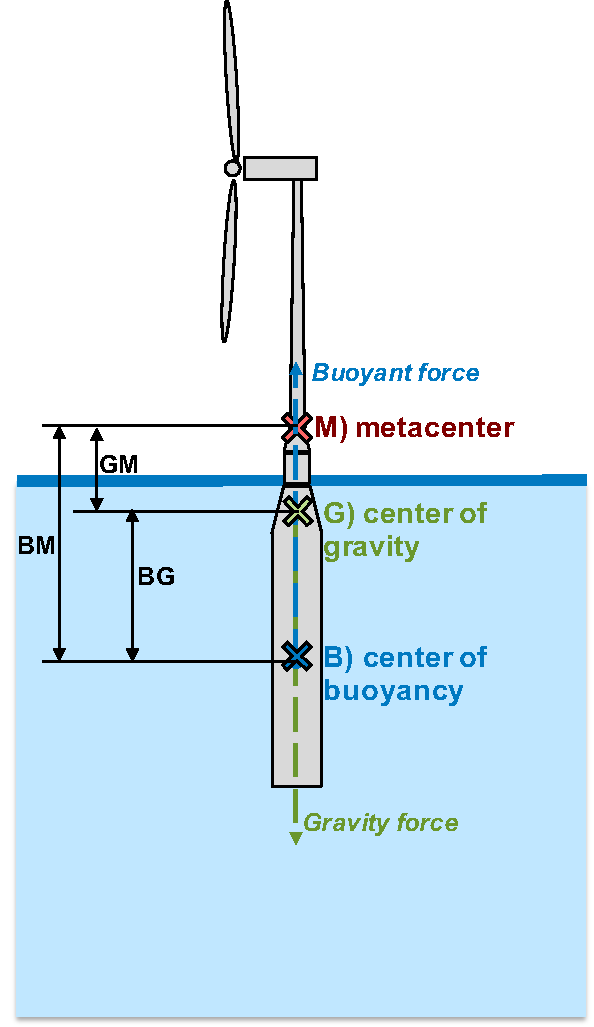
\includegraphics[height=3.5in]{figs/metacenterA.pdf}
    \caption{}
  \end{subfigure}
  \begin{subfigure}[b]{0.49\linewidth}
    \centering 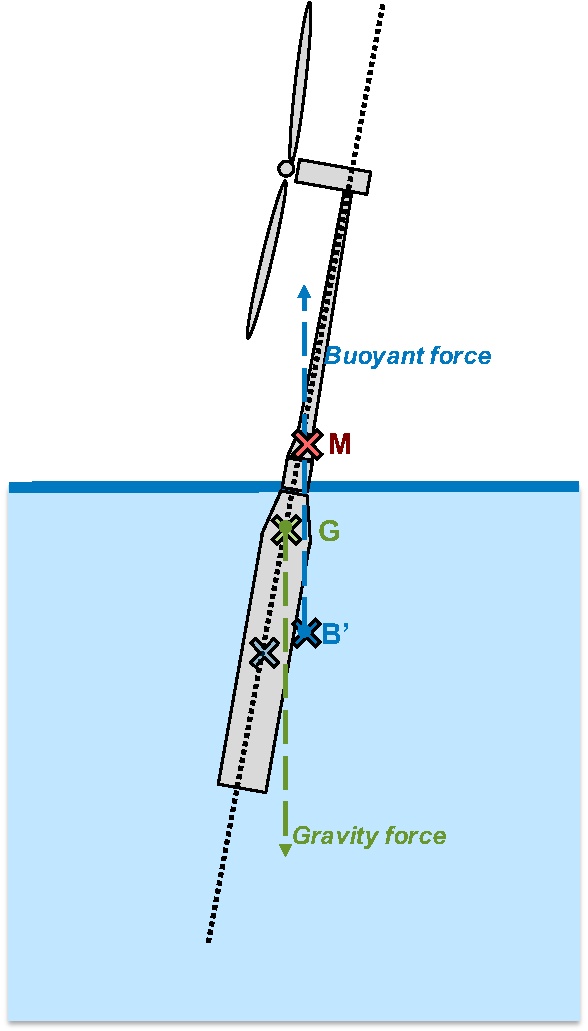
\includegraphics[height=3.5in]{figs/metacenterB.pdf}
    \caption{}
  \end{subfigure}\\
  \caption{Static stability of floating offshore wind turbines.}
  \label{fig:metacenter}
\end{figure}

The second contributing restoring moment comes from the motion of the
center of buoyancy away from alignment with the center of mass.  This is
a standard calculation in naval architecture \citep{thiagarajan2014} and is
diagrammed in Figure \ref{fig:metacenter}.  In this diagram, the center
of mass is denoted, $G$, the center of buoyancy is $B$, and the
metacenter is $M$.  In neural conditions (Figure \ref{fig:metacenter}a),
all of these points are vertically aligned.

As the structure lists or heels, the center of buoyancy shifts toward
the side of the structure that is more submerged (from $B$ to $B'$) and
the buoyancy force no longer passes through the center of mass.
Instead, the buoyancy force passes through the metacenter with an
effective moment arm of $GZ$ from the center of mass (Figure
\ref{fig:metacenter}b).  The metacenter is defined as the common point
through which the buoyancy force acts as it pitches through small
displacements, for bodies with sufficient freeboard margin.

The metacenteric height, $GM$ is most easily calculated as an offset from the
center of buoyancy ($BM$) by,
\[
  h_{meta} = M - G = GM = BM + BG;\quad BM = \frac{I_w}{V}
\]
where $BG$, the distance between the centers of buoyancy and gravity is
easily calculated, $I_w$ is the second moment of area of the substructure waterplane
(with units of \unit{$m^4$}) and $V$ is the total volume of displacement
(with units of \unit{$m^3$}).  Note that for semisubmersible type
geometries, $I_w$ is calculated with the parallel axis theorem for all
of the columns at the waterplane,
\[
  I_w = \sum_i \left( I_{w,i} + S_ir_i^2 \right)
\]
where $S_i$ is the waterplane cross sectional area of the $i$\th column and $r_i$
is the distance from the waterplane centroid to the $i$\th column centroid.

To compute the restoring moment created by the buoyancy force, the first
step is the calculation of the effective moment arm, $GZ$,
\[
GZ = GM \sin \varphi
\]
where $\varphi$ is the angle of heel.  The restoring moment is then the
buoyancy force acting through the restoring arm, $GZ$,
\[
  M_{meta} = F_B \left(GZ\right)
\]
For this reason, the metacenter must be located above the center of mass
for static stability.  This condition is imposed on the design as an
optimization constraint.  Note that the total volume of displacement,
and the subsequent buoyancy force, is not recalculated in the perturbed
configuration.  It is assumed that the angles of deflection are small
and that there is sufficient freeboard and design symmetry such that the
total displacement is constant.

The total restoring pitching moment is then the sum of two
contributions,
\[
  M_{y,restore} = M_{y,moor} + M_{meta}
\]

\section{Hydrostatic Stability}
Floating bodies are typically modeled, for small motions and linearized
behavior, as a second-order differential system with mass, damping, and
spring stiffness terms,
\[
  \left(\mbf{M} + \mbf{A}\right)\ddot{\mbf{x}} + \mbf{C}\dot{\mbf{x}} +
  \mbf{K} = \mbf{F}\left( t \right)
\]
where $\mbf{x}\in\mcal{R}^6$ is the six-degree of freedom vector
(commonly ordered as 1. surge, 2. sway, 3. heave, 4. roll, 5. pitch,
6. yaw), $\mbf{M}$ is the mass matrix, $\mbf{A}$ is the added mass
matrix, $\mbf{C}$ is the damping matrix, and $\mbf{K}$ is the stiffness
matrix.  The right-hand side of the equation captures the time-dependent
summation of all forces.

As a low-fidelity, quasi-static sizing and cost module,
\textit{FloatingSE} does not attempt to capture all of the matrix
entries or forcing terms of the hydrodynamics.  A more sophisticated
time- or frequency-domain solver, where these quantities are calculated, may be linked or included into
\textit{FloatingSE} in the future.  Nevertheless, it does however attempt
to compute the diagonal entries of the mass and stiffness matrices in
order to derive the rigid body natural frequencies of the system,
\[
  \omega_i = \sqrt{\frac{K_{ii}}{M_{ii}+A_{ii}}} \forall i in \left[1\ldots6\right] 
\]
The mass matrix diagonal entries, $M_{ii}$ are simply the mass and
moments of inertia of the whole system,
\[
  M_{11} = M_{22} = M_{33} = m_{sys};\quad M_{44} = I_{xx,sys};\quad M_{55} = I_{yy,sys};\quad M_{66} = I_{zz,sys};
\]
Where the coordinate system notation is consistent with that of Figure
\ref{fig:diagram}.

The added mass matrix diagonal entries are evaluated via standard strip
theory for the tapered columns.  The added mass for the system is a
summation over the columns, using the parallel axis theorem for the
rotational degrees of freedom.  The column quantities are calculated as,
\[
  A_{11} = A_{22} = \rho V;\quad A_{33} = 
  \left(\frac{1}{2}\right)\frac{8}{3} \rho \max R^3(z) ;\quad A_{44} =
  A_{55} = \pi\rho\int\left(z-z_{cb}\right)R^2(z)dz;\quad A_{66} = 0.0;
\]
where $\rho$ is the water density, $R(z)$ is the column radius along its
axis, and $V$ is the submerged volume.  The extra factor of $1/2$ in
$A_{33}$ is included to account for the fact that the top of the column
extends above the waterline.  Also, the integral in $A_{55}$ is only evaluated
along the submerged portion of the column.

The stiffness matrix is comprised of contributions from the mooring
and hydrostatic stiffness.  The mooring linearized stiffness matrix is output
directly from MAP++ and needs no additional processing within
\textit{FloatingSE}.  The hydrostatic stiffness, for a vertical column, is derived from the same
principals described above regarding the metacentric height,
\[
  K_{ii} = K_{ii}^{moor} + K_{ii}^{hydro};\quad K_{33}^{hydro} = \rho g
  S;\quad K_{44}^{hydro} =  K_{55}^{hydro} = \rho g V h_{meta}
\]
where $S$ is the waterplane area of the system.
